\documentclass[a4paper,english,twoside,10pt]{scrreprt}
  \usepackage[utf8]{inputenc}
  \usepackage{babel,geometry,amsmath}
  \usepackage{graphicx,afterpage,float}
  \usepackage[nottoc,numbib]{tocbibind}
  \usepackage[hidelinks]{hyperref}
 % \usepackage[title,titletoc]{appendix}
  \usepackage{fancyhdr}
  \usepackage{listings}								%Used for matlab-code
  \usepackage[framed,numbered,autolinebreaks,useliterate]{mcode} %Used for matlab code
  \setlength{\headheight}{13.6pt}
  \pagestyle{fancy}
  \renewcommand{\chaptermark}[1]{ \markboth{#1}{} }
  \renewcommand{\sectionmark}[1]{ \markright{#1}{} }

  \fancyhf{}
  \fancyfoot[LO,RE]{\thepage}
  \renewcommand{\footrulewidth}{0.4pt}
  %\renewcommand{\headrulewidth}{0pt} 
  \fancyhead[RE]{\textit{ \nouppercase{\leftmark}} }
  \fancyhead[LO]{\textit{ \nouppercase{\rightmark}} }

  \fancypagestyle{plain}{ %
    \fancyhf{} % remove everything
    \fancyfoot[LO,RE]{\thepage}
    \renewcommand{\headrulewidth}{0pt} % remove lines as well
    %\renewcommand{\footrulewidth}{0pt}
  }

  \renewcommand{\chapterheadstartvskip}{\vspace *{0.1\baselineskip }}

  \makeatletter
\g@addto@macro\appendix{%
  \renewcommand*{\chapterformat}{%
    {\chapapp\nobreakspace\thechapter\autodot\enskip}%
  }
  \renewcommand*{\chaptermarkformat}{%
    {\chapapp\nobreakspace\thechapter\autodot\enskip}%
  }
  \let\oldaddcontentsline\addcontentsline
  \newcommand\hackedaddcontentsline[3]{\oldaddcontentsline{#1}{#2}{\chapapp\nobreakspace#3}}
  \let\oldchapter\chapter
  \renewcommand*\chapter[1]{%
    \let\addcontentsline\hackedaddcontentsline%
    \oldchapter{#1}%
    \let\addcontentsline\oldaddcontentsline%
  }
}
\makeatother

\begin{document}

  \begin{titlepage}

	\begin{center}~
		\\[5cm]

		
\includegraphics[width=0.4\textwidth]{./img/logontnu}~
		\\[0.3cm]
		\textsc{ Department of Electronics and Telecommunications}~
		\\[2cm]

		{ \huge \bfseries TTT4115 Kommunikasjonsteori Vår 2015 \\[0.5cm]
		Semesterproject spring 2015 }~
		\\[1.5cm]
		

		{ \LARGE Helge Langen, Lars-Arne Larsen}
	\end{center}


\end{titlepage}

  \clearpage
  \setcounter{page}{1}

  \tableofcontents	
  \clearpage

  \chapter{Problem 1}
  \section{Problem 1a}
	
	From the z-transform of the described filter in Problem 1 we get:
	\begin{equation}
		X(z)=\rho X(z)z^{-1}+\sqrt{1-\rho ^2}*E(z) 
		\label{eq:eq_impulse_response}
	\end{equation}
	If we sort equation~\ref{eq:eq_impulse_response} in regard of $\frac{X(z)}{E(z)}$ we get:
	\begin{equation*}
		\frac{X(z)}{E(z)}=\frac{\sqrt{1-\rho ^2}}{1-\rho z^{-1}}
		\label{eq:eq_freq_resp_x}
	\end{equation*}
	
	Make the z-transform back to the diskrete plane
	
	\begin{equation*}
		h(n)=\sqrt{1-\rho ^2}\rho ^nu(n)
	\end{equation*}
	
	Since the noise is uncorrolated, we may reduce the convolution to find x(n)
	
	\begin{equation*}
		x(n)=h(n)\Asterisk e(n)=h(n)\sigma ^2_W
	\end{equation*}
	
	From Problem 1 it is given that
	
	\begin{equation*}
		\sigma ^2_W=1
	\end{equation*}
	
	This results in the following expression for x(n):
	
	\begin{equation}
		x(n)=\sqrt{1-\rho ^2}\rho ^nu(n)
		\label{eq:eq_AR_process}
	\end{equation}
	
	From the output calculated in equation~\ref{eq:eq_AR_process} we may use the following formula from the compendium to calculate the autocorrelation:
	
	\begin{equation}
		R_x(\tau)=\sum_{n=-\infty}^{\infty}E\{x(n)\}E\{x(n+\tau)\}
		\label{eq:eq_autocorrelation_compendium}
	\end{equation}
	
	By inserting our definition of x(n) we get the following equation:
	
	\begin{equation*}
		R_x(\tau)=(1-\rho ^2)\sum_{n=0}^{\infty}\rho ^n\rho^{n+\tau}
	\end{equation*}
	
	By using the formula for geometric series we conclude with this resulting formula:
	
	\begin{equation*}
		R_x(\tau)=(1-\rho ^2)\rho^{\tau }\sum_{n=0}^{\infty}\rho^{2n}=(1-\rho ^2)\rho^{\tau }\frac{1}{1-\rho ^2}
	\end{equation*}
	
	After shorting down the last equation, this is the complete answer:
	
	\begin{equation}
		R_x(\tau)=\rho^{|\tau |}
	\end{equation}
	
	\lstinputlisting{Matlab/oppgave1a.m}
	
	\begin{figure}[H]
	  \centering
	  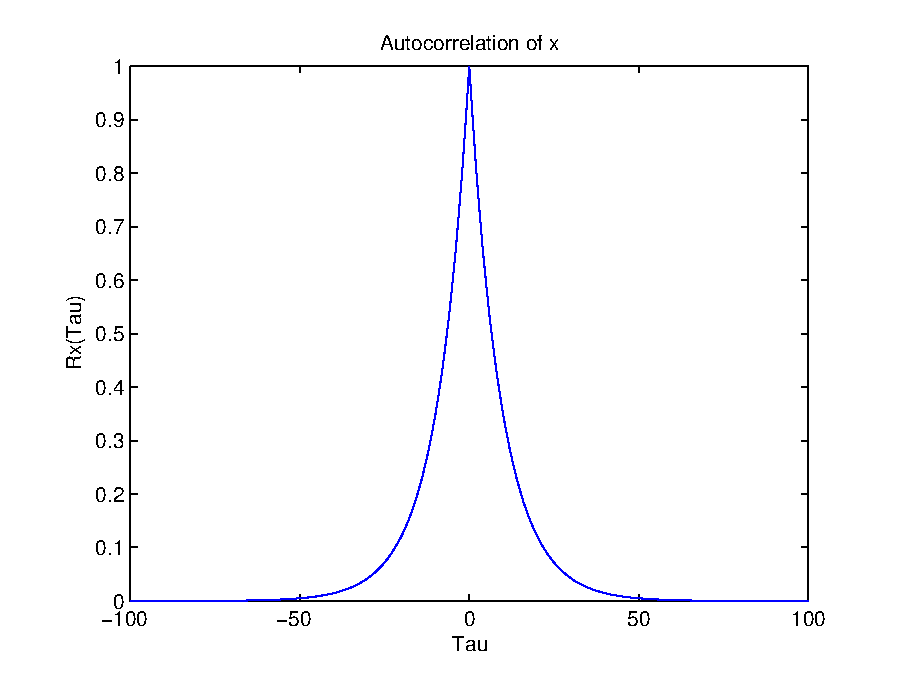
\includegraphics[width=0.75\textwidth]{img/Oppgave1a}
	\end{figure}
	
  
  
  \section{Problem 1b}
	From the compendium we have that the power spectral density may be given by the following formula:
	\begin{equation}
		Sx(f)=|H(f)|^2=H(f)H^*(f)
	\end{equation}
	
	Insert the expression from equation~\ref{eq:eq_freq_resp_x} and calculate:
	
	\begin{equation*}
		H(f)=H(z)|_{z=e^{j2\pi f}}=\frac{\sqrt{1-\rho ^2}}{1-\rho e^{-j2\pi f}}
	\end{equation*}
	
	Expanding the denominator and cleaning up.
	
	\begin{equation*}
		Sx(f)=\frac{\sqrt{1-\rho ^2}^2}{(1-\rho e^{-j2\pi f})(1-\rho e^{j2\pi f})}=\frac{1-\rho ^2}{1-\rho e^{j2\pi f}-\rho e^{-j2\pi f}+\rho ^2}
	\end{equation*}
	
	Using eulers formula for cosine function to reduce the equation to the following result:
	
	\begin{equation}
		Sx(f)=\frac{1-\rho ^2}{1+\rho ^2-2\rho cos(2\pi f)}
		\label{eq:eq_Spectral_Density_X}
	\end{equation}
	
	\lstinputlisting{Matlab/Oppgave1b.m}
	
	\begin{figure}[H]
	  \centering
	  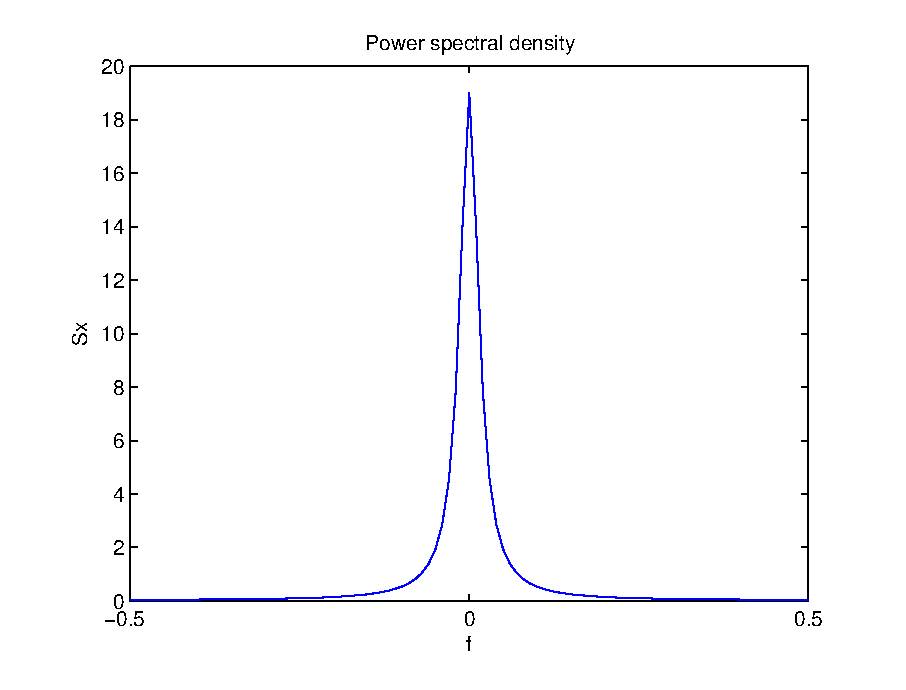
\includegraphics[width=0.75\textwidth]{img/Oppgave1b}
	\end{figure}
  
  \section{Problem 1c}
  
	\lstinputlisting{Matlab/Oppgave1c.m}
  
  \section{Problem 1d}
  
	\lstinputlisting{Matlab/Oppgave1d.m}
	
	\begin{figure}[h]
	  \centering
	  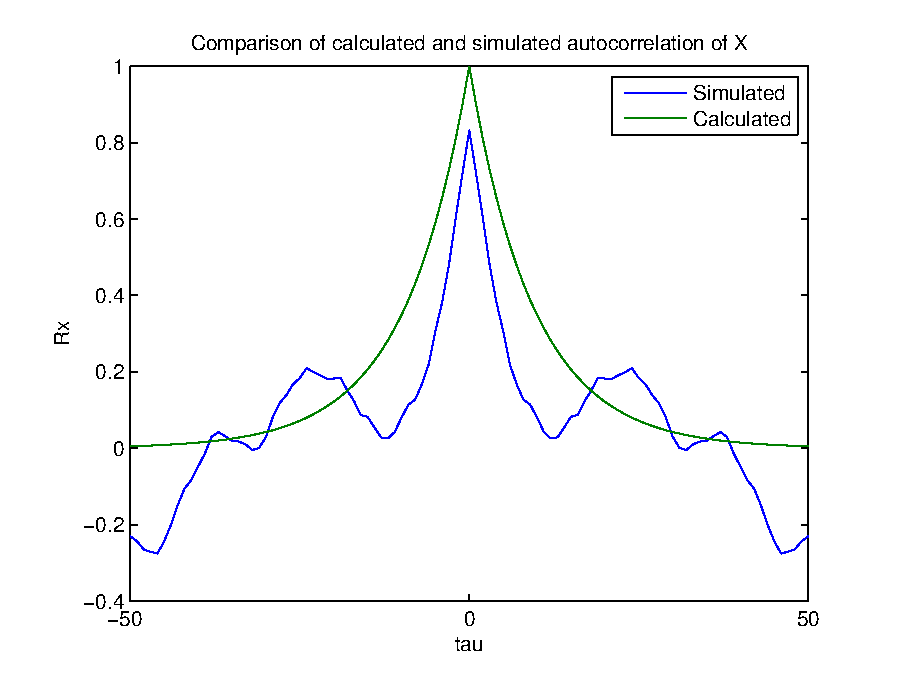
\includegraphics[width=0.75\textwidth]{img/Oppgave1d}
	\end{figure}
  
  \section{Problem 1e}
  
	\lstinputlisting{Matlab/Oppgave1e.m}
	
	\begin{figure}[h]
	  \centering
	  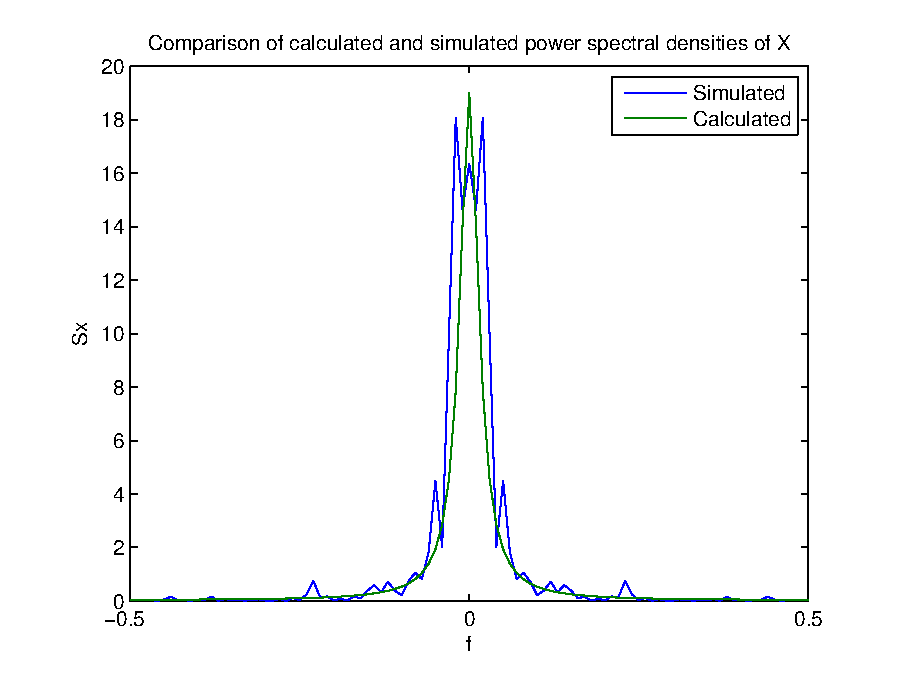
\includegraphics[width=0.75\textwidth]{img/Oppgave1e}
	\end{figure}

  \chapter{Problem 2}
To shorten the length of this report, the code for problem 2 have been put together instead of having seperate code for a, b and c which may be found in \ref{app:2}. All plots made in normalized frequency have been from $0$ to $\frac{1}{2}$ since they are real functions. Since the functions are real, the frequency plot is even, and easier to interpret this way.
                          
\section{Problem 2a}
	
	
	Equation~\ref{eq:eq_bit_rate} for bitrate was given in the exercise 
	\begin{equation}
		H=\frac{1}{2}log(2\pi e^1\frac{\sigma ^2 _U}{\Delta ^2})
		\label{eq:eq_bit_rate}
	\end{equation}
	
	Solved equation~\ref{eq:eq_bit_rate} for $\Delta ^2$ for use in later equations
	
	\begin{equation}
		\Delta ^2=\frac{2\pi e^1\sigma ^2 _U}{2^{2H}}
		\label{eq:step_size}
	\end{equation}
	
	Equation~\ref{eq:eq_lagrange_mult} is equation (3.15) from the compendium and is used in the process of calculating the optimal filters.
	
	\begin{equation}
		\sqrt{\lambda}=\frac{\int\limits_{-\infty}^{\infty}\sqrt{S_x(f)S_Q(f)}df}{P+\sigma^2_Q}
		\label{eq:eq_lagrange_mult}
	\end{equation}
	
	For the calculation of the lagrange multiplier, equation~\ref{eq:step_from_noise} is given in the exercise:
	
	\begin{equation}
		\sigma^2_Q=\frac{\Delta^2}{12}
		\label{eq:step_from_noise}
	\end{equation}
	
	The noise is constant over the frequency-band, thus applying
	
	\begin{equation*}
		S_N(f)=\sigma^2_Q
	\end{equation*}
	
	All inserted in equation~\ref{eq:eq_lagrange_mult} gives equation~\ref{eq:lagrange_full}.

	\begin{equation}
		\sqrt{\lambda}=\frac{\int\limits_{-\frac{1}{2}}^{\frac{1}{2}}\sqrt{\frac{0.19\sigma^2_Q}{1.81-1.8cos(2\pi f)}}df}{1+\sigma^2_Q}
		\label{eq:lagrange_full}
	\end{equation}
	
	The integral in equation~\ref{eq:lagrange_full} had to be solved numerically using matlab. The calculated functions and values are used in equation~\ref{eq:optimal_receiver} and ~\ref{eq:optimal_transmitter} to calculate the optimal transmitter/receiver filters.
	
	\begin{equation}
		|H(f)|^2=\sqrt{\frac{\lambda S_x(f)}{S_N(f)}}-\lambda
		\label{eq:optimal_receiver}
	\end{equation}
	
	\begin{equation}
		|G(f)|^2=\sqrt{\frac{S_N(f)}{\lambda S_x(f)}}-\frac{S_N(f)}{S_x(f)}
		\label{eq:optimal_transmitter}
	\end{equation}
	
	The resulting frequency responses for the filters are shown in figure~\ref{fig:freq_opt_G} and \ref{fig:freq_opt_H}.
	
	\begin{figure}[H]
	  \centering
	  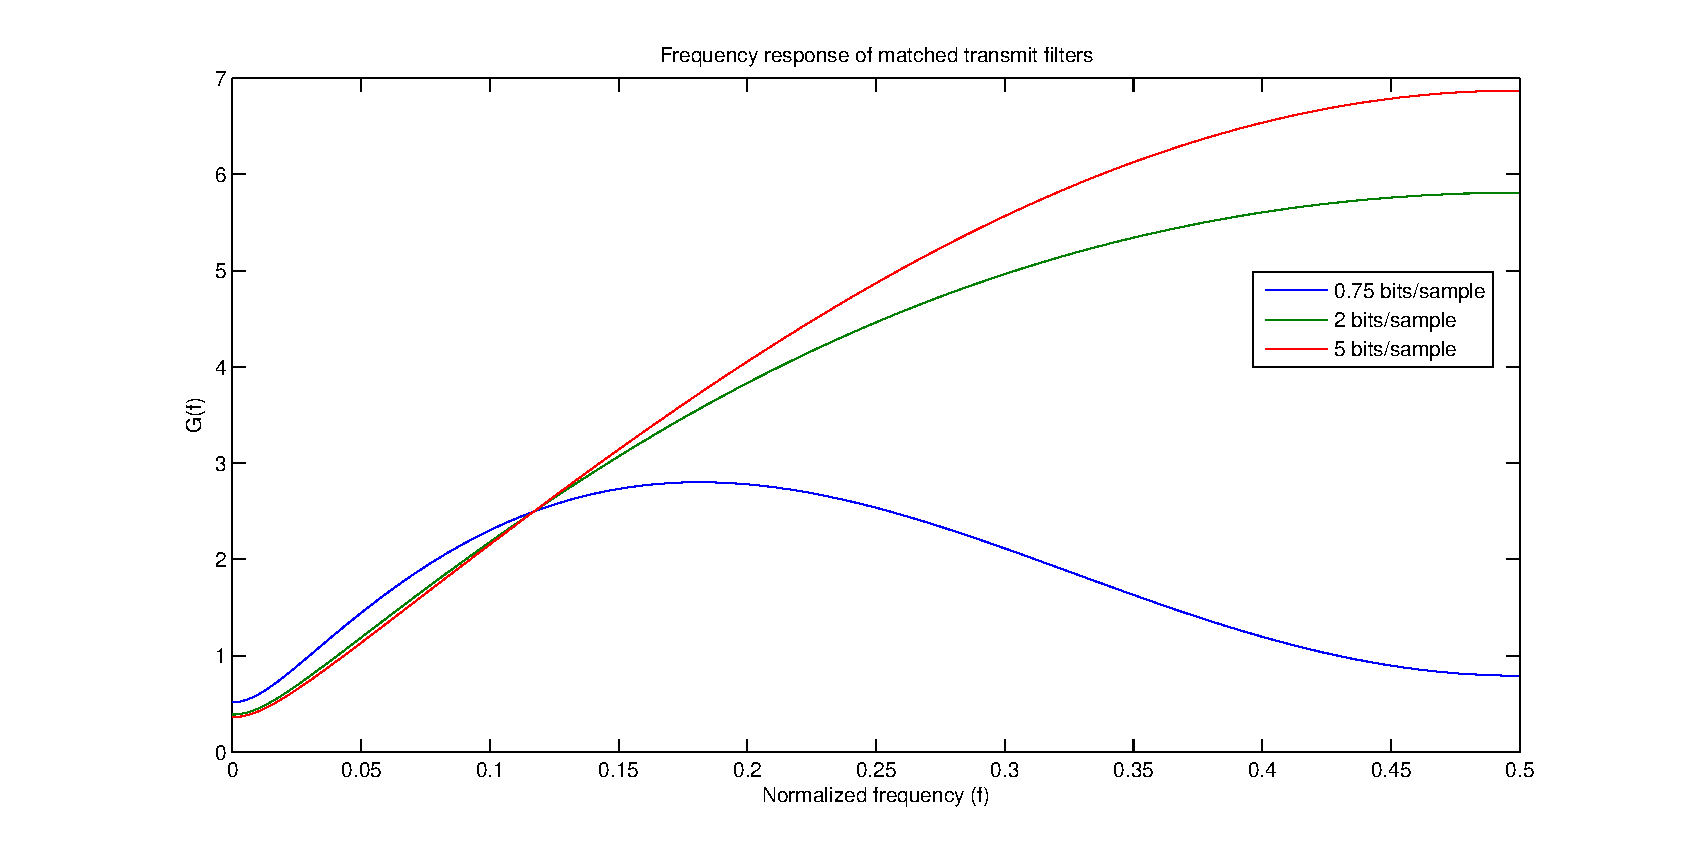
\includegraphics[width=0.75\textwidth]{img/Oppgave2a_freq_G}
	  \label{fig:freq_opt_G}
	  \caption{Frequency response of transmit filter}
	\end{figure}
	
	\begin{figure}[H]
	  \centering
	  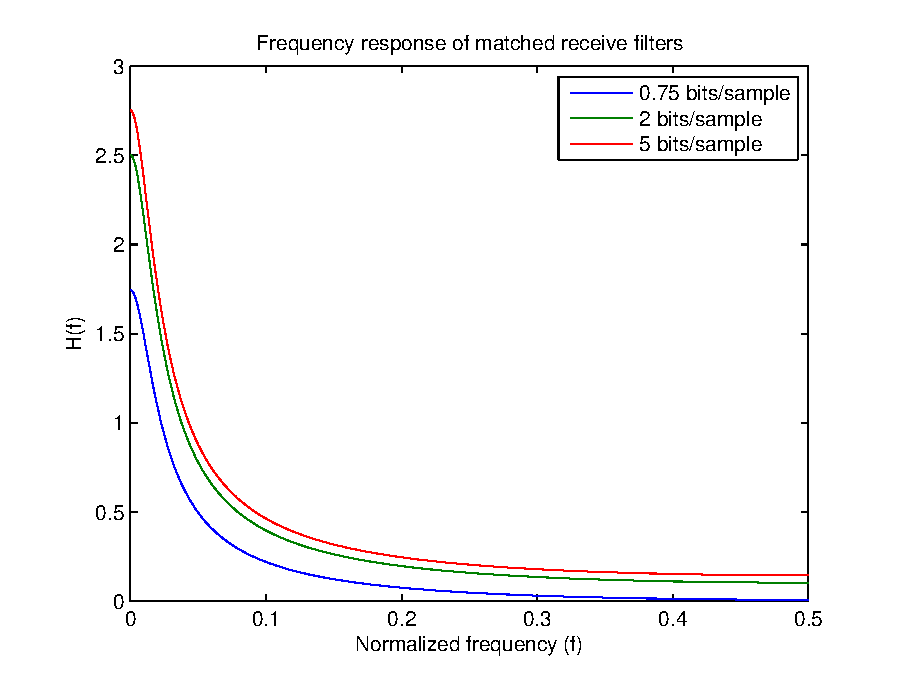
\includegraphics[width=0.75\textwidth]{img/Oppgave2a_freq_H}
	  \label{fig:freq_opt_H}
	  \caption{Frequency response of receiver filter}
	\end{figure}
	
	To calculate the power spectral densities of the output noise and signal component, they where first calculated seperatly by using equation~\ref{eq:noise_out_spec} and ~\ref{eq:sig_out_spec}. The results are shown in figure~\ref{fig:sig_noise_freq_out}
	
	\begin{equation}
		N(f)=\sigma _Q^2|H(f)|^2
		\label{eq:noise_out_spec}
	\end{equation}
	
	\begin{equation}
		Y(f)=S_x(f)|G(f)|^2|H(f)|^2
		\label{eq:sig_out_spec}
	\end{equation}
	
	
	\begin{figure}[H]
	  \centering
	  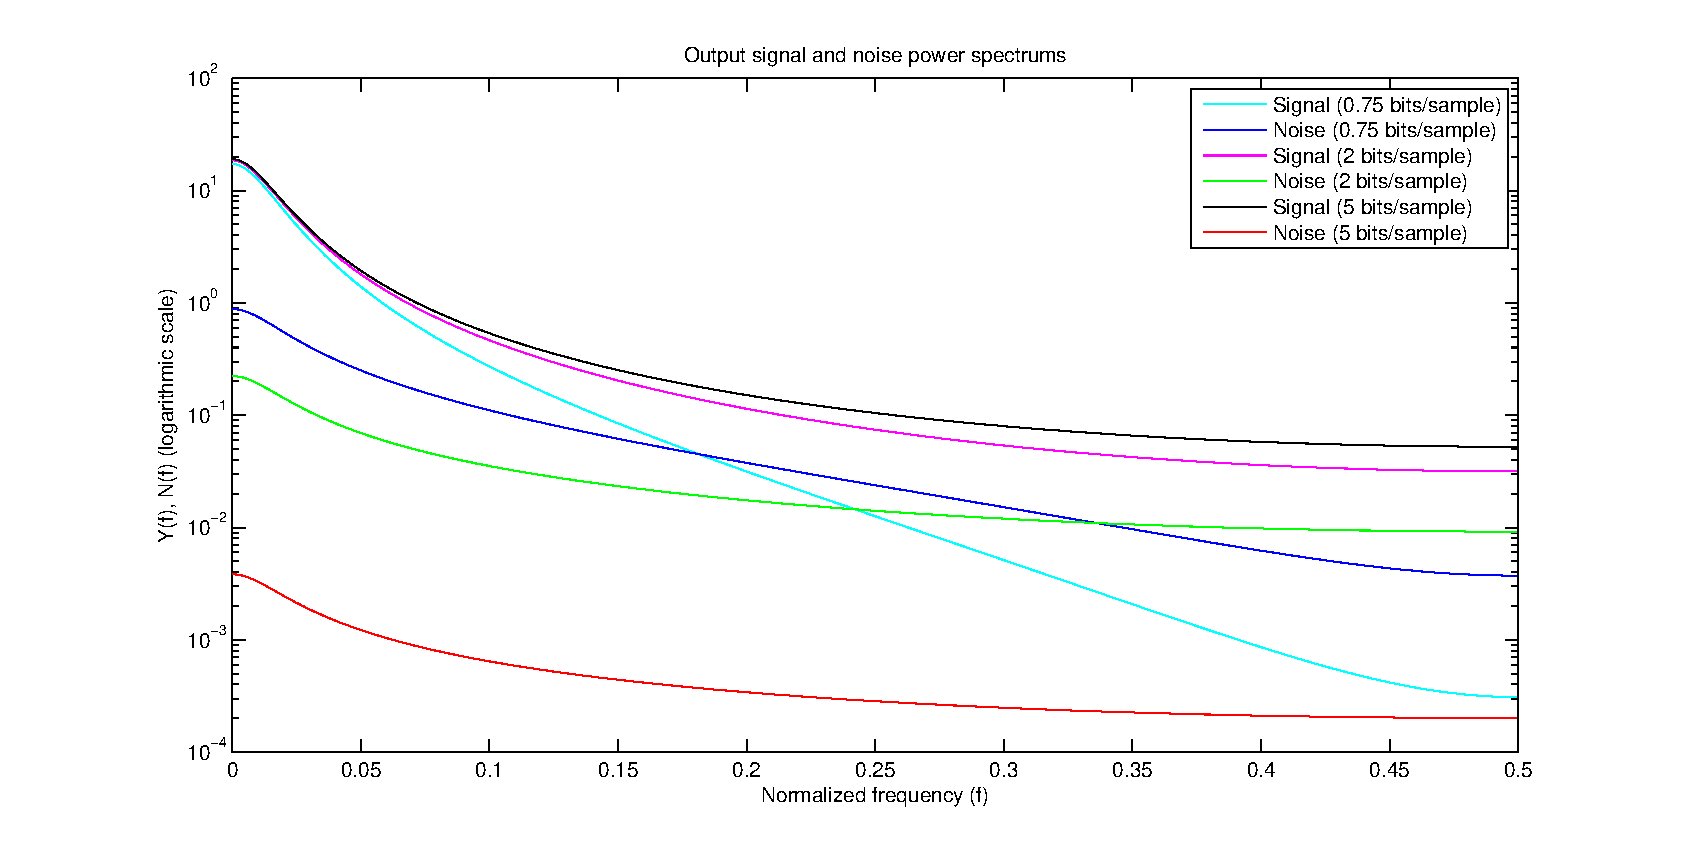
\includegraphics[width=0.75\textwidth]{img/Oppgave2a_sig_noise_freq_out}
	  \label{fig:sig_noise_freq_out}
	  \caption{Output signal and noise power spectrum}
	\end{figure}
	
	To calculate the SNR, spectras shown in  figure~\ref{fig:sig_noise_freq_out} si used as shown in equation~\ref{eq:SNR}
	
	\begin{equation}
		SNR=10log\left(\frac{\int\limits_{-\frac{1}{2}}^{\frac{1}{2}}Y(f)df}{\int\limits_{-\frac{1}{2}}^{\frac{1}{2}}N(f)df}\right)
		\label{eq:SNR}
	\end{equation}
	
	The estimated values for the different bitrates is shown in table~\ref{tab:SNR_results}
	
	\begin{table}[H]
		\centering
		\begin{tabular}{l l l l}
			H[bits/sample] & noise power($\sigma^2_Q$) & Lagrange ($\lambda$) & SNR[dB] \\
			0.75 & 0.532 & 0.0892 & 9.45 \\
			2 & 0.0890 & 0.03 & 14.99 \\
			5 & 0.0014 & 0.00055 & 32.60 \\
		\end{tabular}
		\label{tab:SNR_results}
		\caption{Shows SNR values for different bitrates.}
	\end{table}

\section{Problem 2b}
	The function FrSamp() that was given in the exercise was used to make an inverse fft of the receive and transmit filters. The inverse fft of a frequency respones will be the same as the impulse response to the given function. Higher resolution of the inverse fft will increase the resolution of the impulse response. The impulse response of the receive and transmit filters are shown in figure~\ref{fig:impulse_G_diskrete} and ~\ref{fig:impulse_H_diskrete}.
	
	\begin{figure}[h]
	  \centering
	  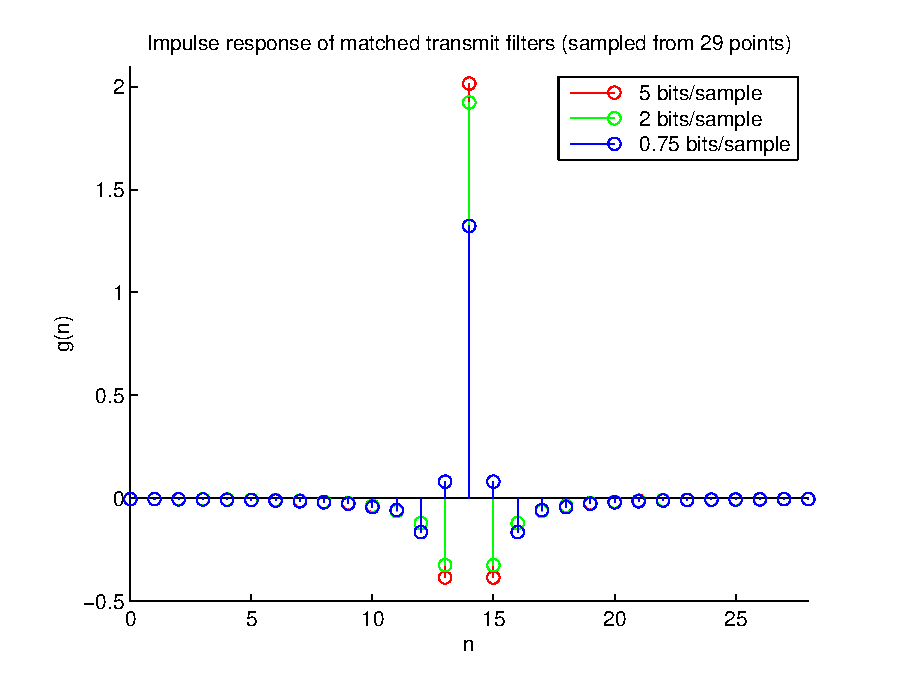
\includegraphics[width=0.9\textwidth]{img/Oppgave2b_impulse_G_diskrete_t}
	  \label{fig:impulse_G_diskrete}
	  \caption{Impulse response of transmit filter}
	\end{figure}
	
	\begin{figure}[h]
	  \centering
	  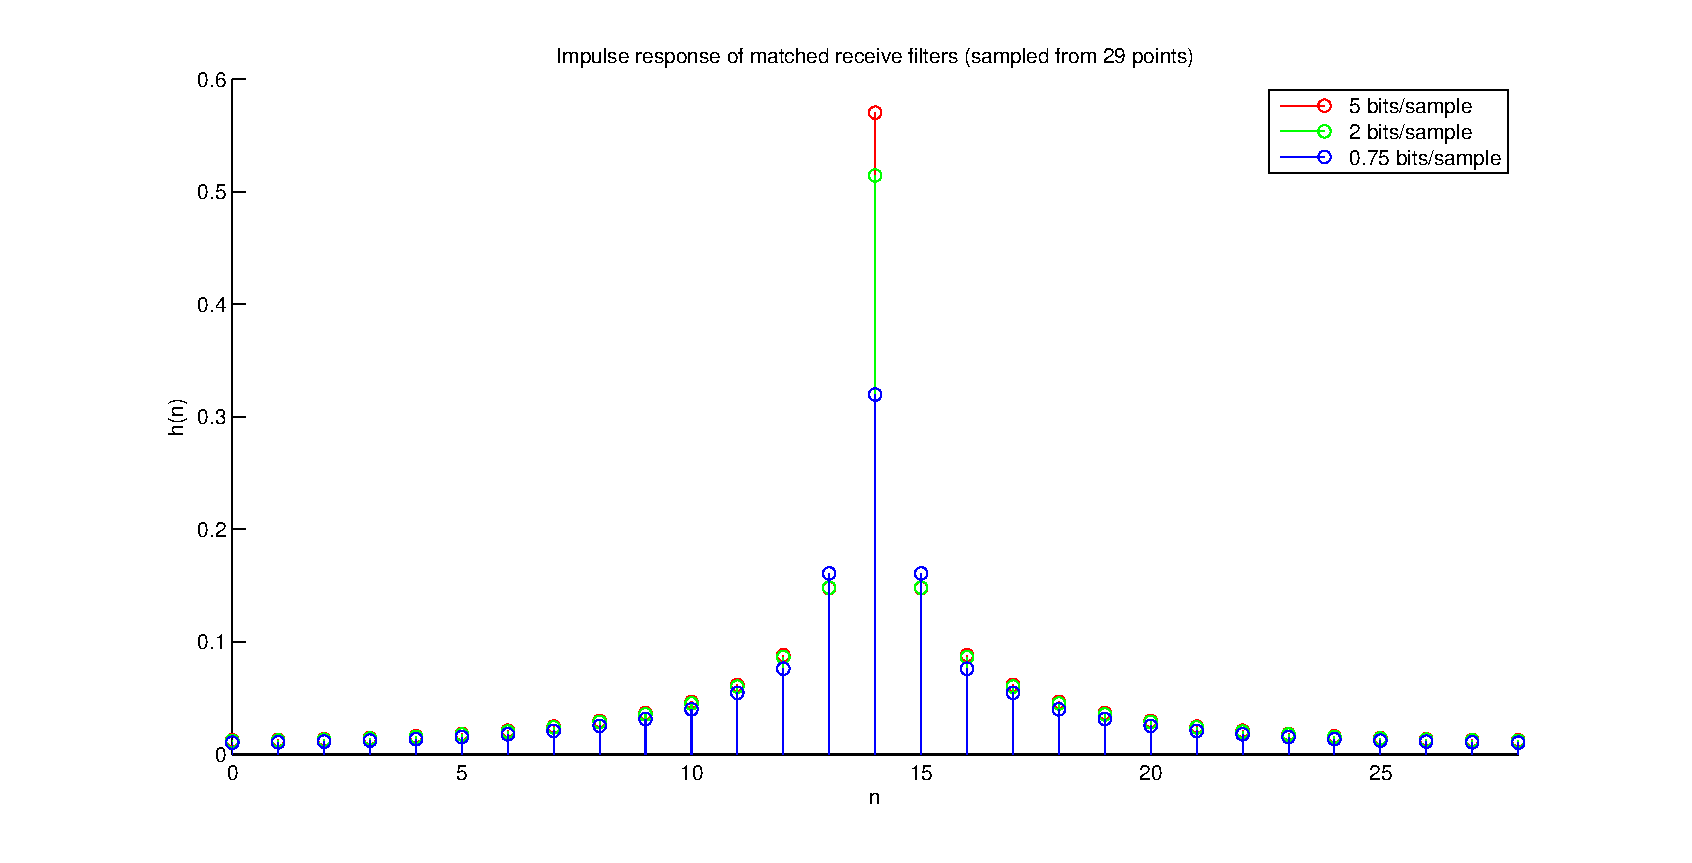
\includegraphics[width=0.9\textwidth]{img/Oppgave2b_impulse_H_diskrete_t}
	  \label{fig:impulse_H_diskrete}
	  \caption{Impulse response of receiver filter}
	\end{figure}
	
	To be able to compare the calculated and the exact filters, an fft is done on the impulse responses shown in figure~\ref{fig:impulse_G_diskrete} and ~\ref{fig:impulse_H_diskrete}. The comparison of exact and calculated filters are shown in figure~\ref{fig:freq_comp_G} and figure~\ref{fig:freq_comp_H}.
	
	\begin{figure}[h]
	  \centering
	  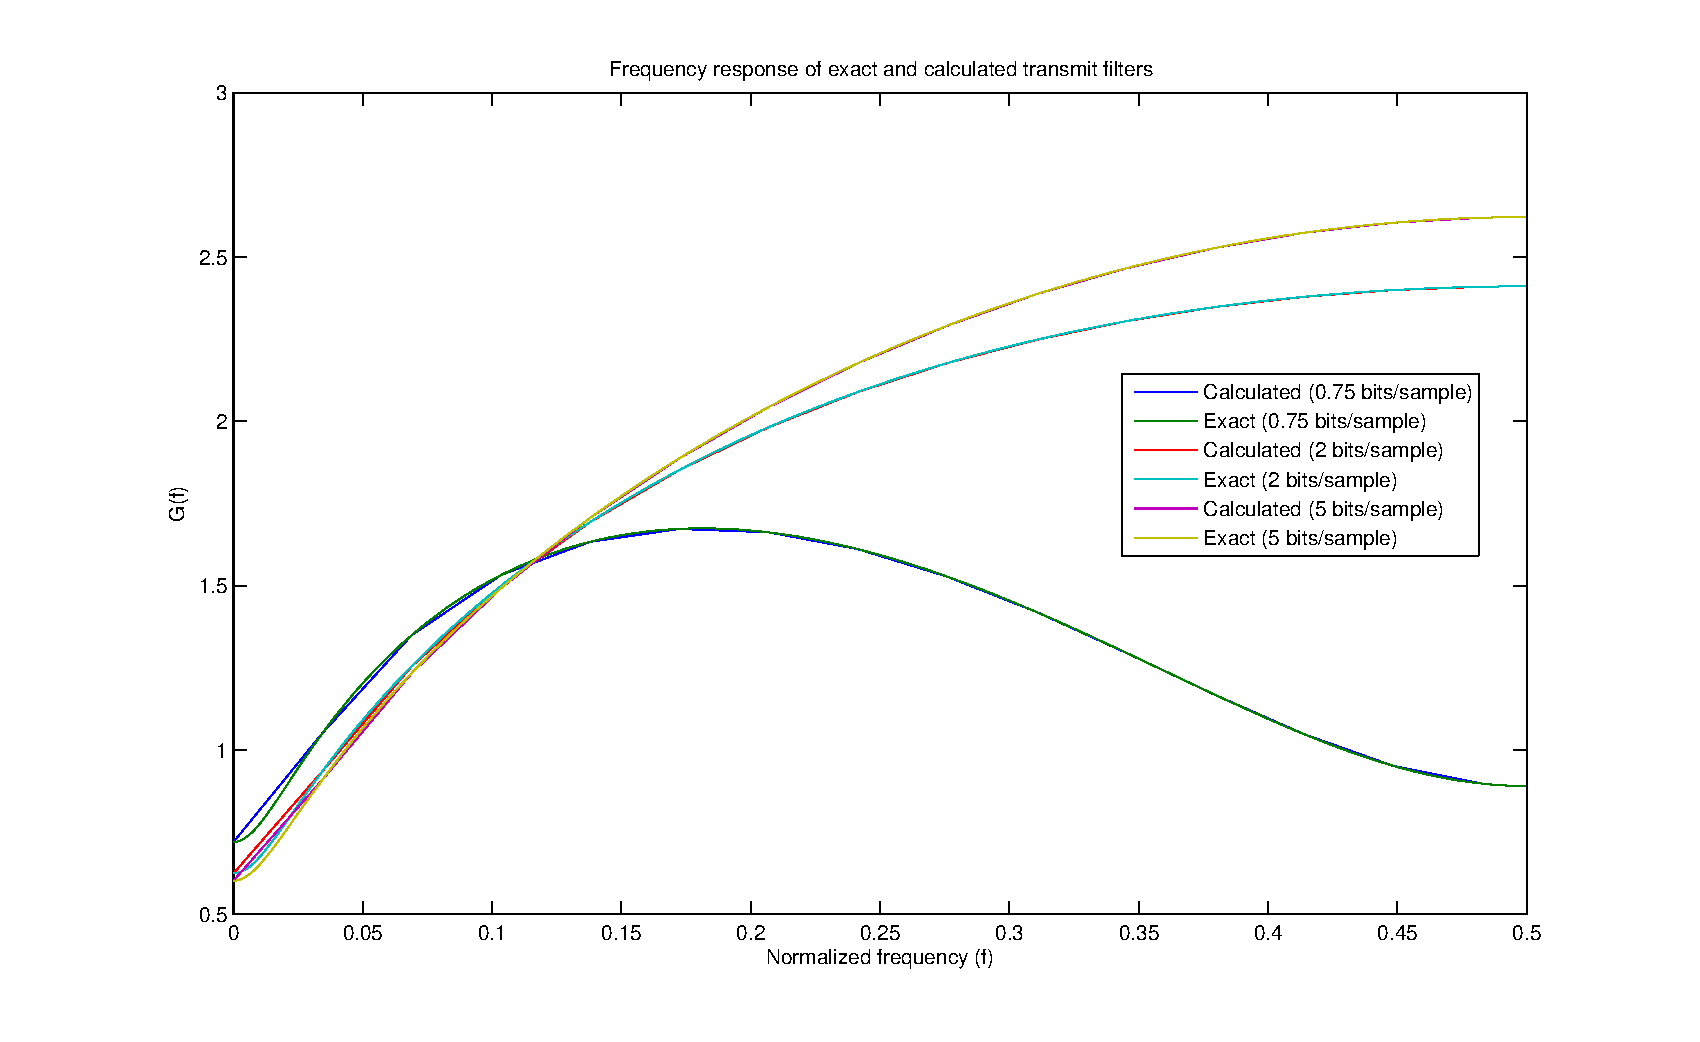
\includegraphics[width=0.9\textwidth]{img/Oppgave2b_freq_G}
	  \caption{Comparison of calculated and exact transmit filters}
	  \label{fig:freq_comp_G}
	\end{figure}
	
	\begin{figure}[h]
	  \centering
	  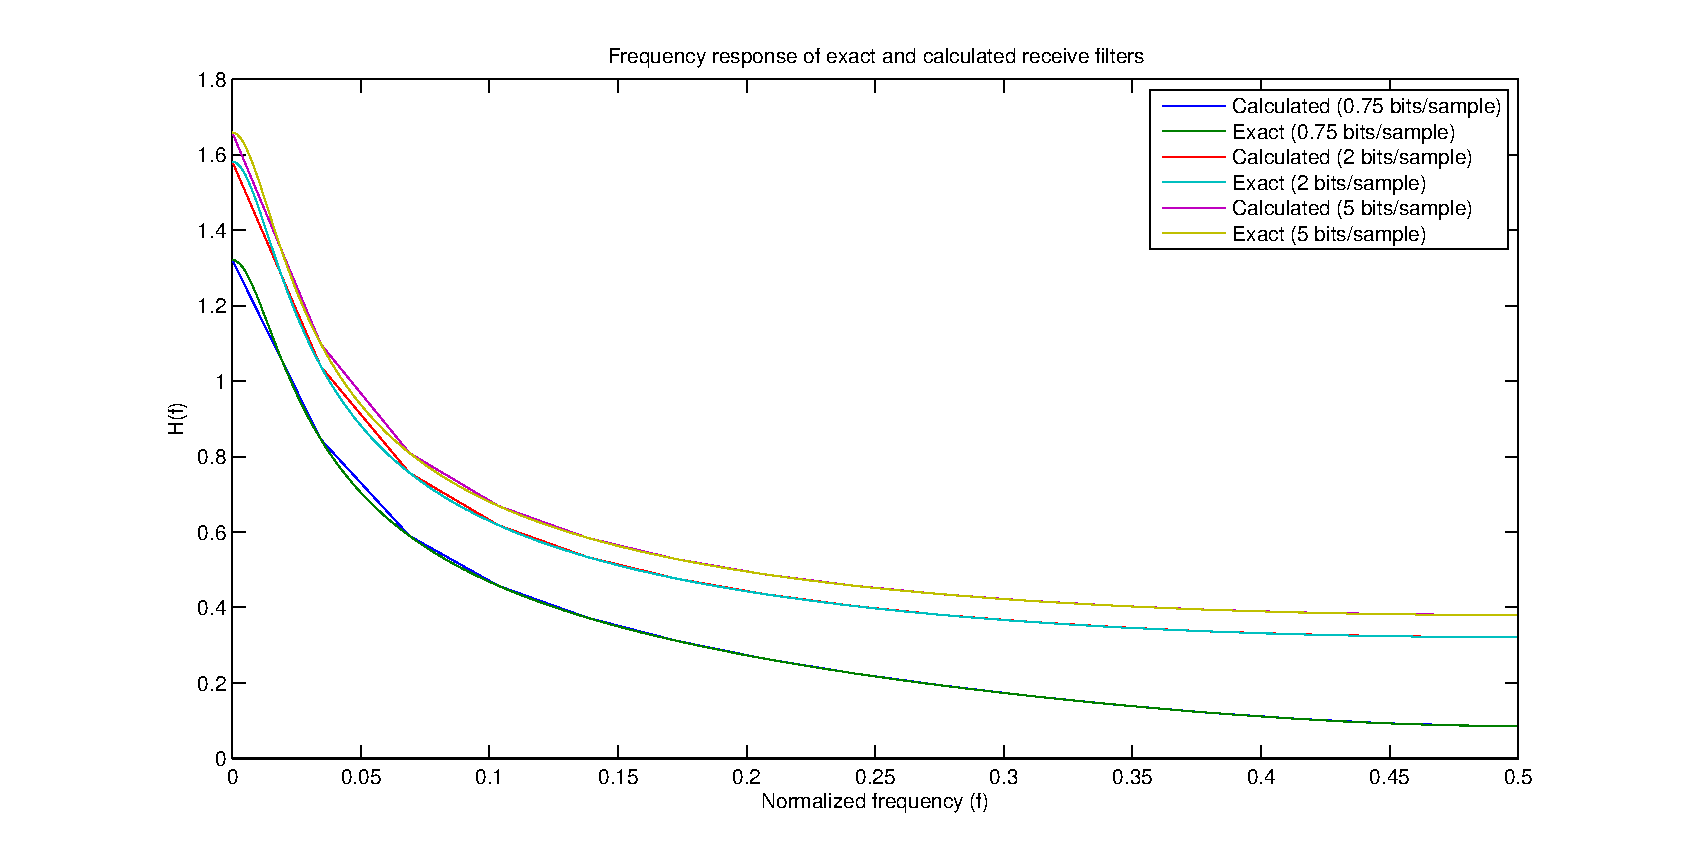
\includegraphics[width=0.9\textwidth]{img/Oppgave2b_freq_H}
	  \caption{Comparison of calculated and exact receive filters}
	  \label{fig:freq_comp_H}
	\end{figure}
	
	To show how the signal is modified through the system, equation 3.19 from the compendium is used. The equation is shown in equation~\ref{eq:total_sig_mod} and the result is plotted in figure~\ref{fig:signal_mod_xy}.
	
	\begin{equation}
		|H(f)G(f)|=1-\sqrt{\lambda \frac{S_N(f)}{S_x(f)}}
		\label{eq:total_sig_mod}
	\end{equation}
	
	\begin{figure}[h]
	  \centering
	  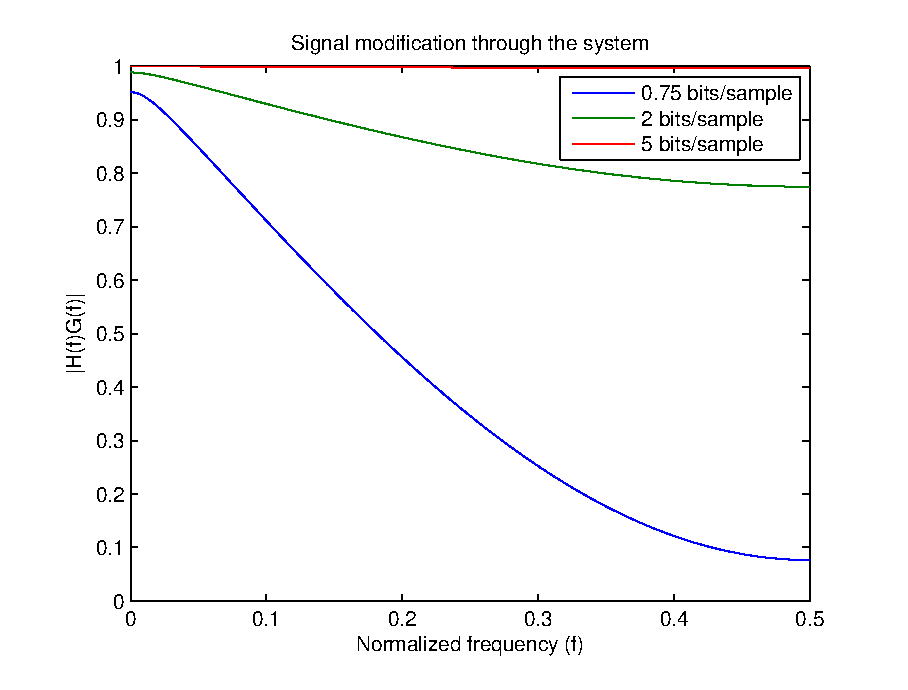
\includegraphics[width=0.9\textwidth]{img/Oppgave2b_signal_mod_x_y}
	  \label{fig:signal_mod_xy}
	  \caption{Signal modification through the system}
	\end{figure}

\section{Problem 2c}
	
	To measure the bitrate, we had to decide step size from equation~\ref{eq:step_from_noise} and use this to decide decision limits and representation levels. Then the output signal from G(f) where quantized using the quantiz() function from communication systems toolbox and shown in figure~\ref{fig:Quant_output}.
	
	\begin{figure}[h]
		\centering
		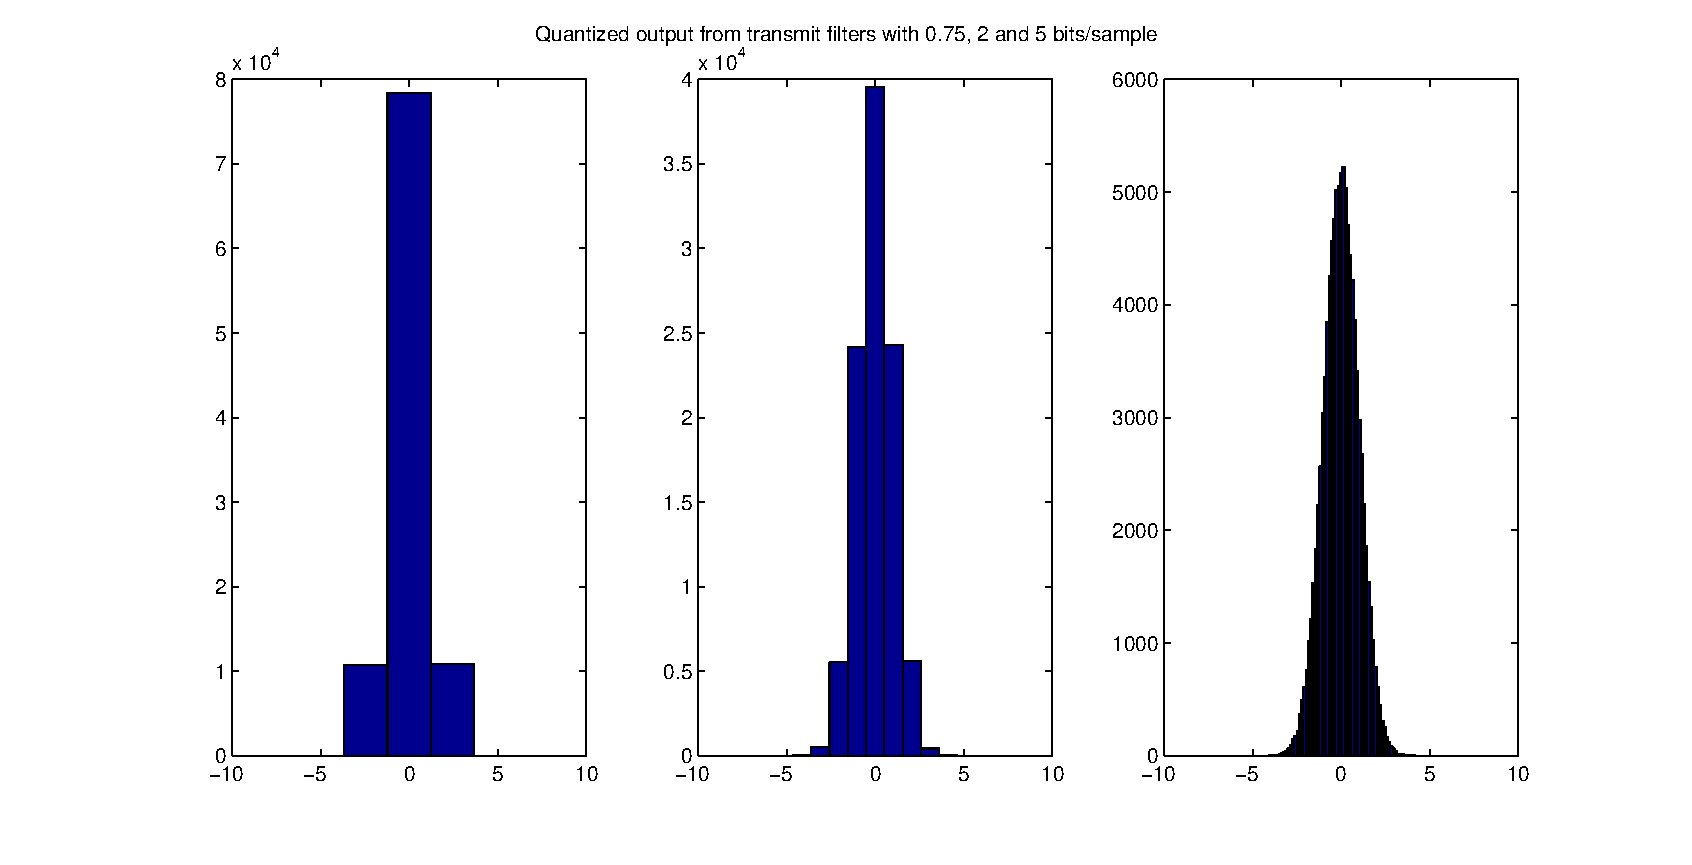
\includegraphics[width=0.9\textwidth]{img/Oppgave2c_Quant_output}
		\label{fig:Quant_output}
		\caption{Quantized output from transmit filters with 0.75, 2 and 5 bits/sample}
	\end{figure}
	The upper and lower quantization limits were decided from figure~\ref{fig:Quant_output} so that we did not truncate any levels. 
	
	The definition for bitrate is given in the exercise and is shown in equation~\ref{eq:bitrate_def} where $P_i$ is the probability of being inside interval i. The results from calculation is given in table~\ref{tab:result_SNR_H}.
	
	\begin{equation}
		H=-\sum\limits_{i=1}^{I}P_ilog_2(P_i)
		\label{eq:bitrate_def}            
	\end{equation}
	
	\begin{table}[h]
		\centering
		\begin{tabular}{l l l l l}
			H[bit/symbol] & SNR theoretical[dB] & SNR simulated[dB] & Step size($\Delta$) & H simulated[bit/symbol]\\
			0.75 & 9.45 & 7.49 & 2.4573 & 0.97 \\
			2 & 14.99 & 14.78 & 1.0332 & 2.06\\
			5 & 32.60 & 29.69 & 0.1291 & 4.99\\
		\end{tabular}
		\label{tab:result_SNR_H}
	\end{table}
	
	As seen in table~\ref{tab:result_SNR_H}, the simulated bitrate deviates from the given one for low bitrates. This result complies with the exercise text where it is stated that the equation~\ref{eq:eq_bit_rate} is for high-rate systems. 
	
	We noted that the SNR would improve if length of filters are increased.	
  
\end{document}
